% This must be in the first 5 lines to tell arXiv to use pdfLaTeX, which is strongly recommended.
\pdfoutput=1
% In particular, the hyperref package requires pdfLaTeX in order to break URLs across lines.

\documentclass[11pt]{article}

\usepackage[table]{xcolor}

% Remove the "review" option to generate the final version.
\usepackage[]{style/acl2023}

% Standard package includes
\usepackage{times}
\usepackage{latexsym}
\usepackage{amsmath}
\usepackage{amssymb}
\usepackage{amsthm}
\usepackage{relsize}
\usepackage{dsfont}
\usepackage{graphicx}
\usepackage{float}
% For proper rendering and hyphenation of words containing Latin characters (including in bib files)
\usepackage[T1]{fontenc}
% For Vietnamese characters
% \usepackage[T5]{fontenc}
% See https://www.latex-project.org/help/documentation/encguide.pdf for other character sets

% This assumes your files are encoded as UTF8
\usepackage[utf8]{inputenc}

% This is not strictly necessary, and may be commented out.
% However, it will improve the layout of the manuscript,
% and will typically save some space.
\usepackage{microtype}

% This is also not strictly necessary, and may be commented out.
% However, it will improve the aesthetics of text in
% the typewriter font.
\usepackage{inconsolata}

%%%%%%%%%%%%%%%%%%%%%%%%%%%%%%%%%%%%%%%%%%%
%%%%%% Specify Custom Packages below %%%%%%
%%%%%%%%%%%%%%%%%%%%%%%%%%%%%%%%%%%%%%%%%%%

\usepackage{hyperref}
\usepackage{bm}

\usepackage{algorithm}
\usepackage[noend]{algpseudocode}
\usepackage{tabularx}

% \usepackage{stfloats}
\usepackage{indentfirst}


% If the title and author information does not fit in the area allocated, uncomment the following
%
%\setlength\titlebox{<dim>}
%
% and set <dim> to something 5cm or larger.

\title{Exploring Extractive and Abstractive Approaches for Multi-Document Summarization: An End-to-End System with Benchmarking and Error Analysis}

% Author information can be set in various styles:
% For several authors from the same institution:
\author{Anna Batra, Sam Briggs, Junyin Chen, Hilly Steinmetz\\
          Department of Linguistics, University of Washington \\
          \texttt{\{batraa, briggs3, junyinc, hsteinm\}@uw.edu}}
% if the names do not fit well on one line use
%         Author 1 \\ {\bf Author 2} \\ ... \\ {\bf Author n} \\
% For authors from different institutions:
% \author{Author 1 \\ Address line \\  ... \\ Address line
%         \And  ... \And
%         Author n \\ Address line \\ ... \\ Address line}
% To start a seperate ``row'' of authors use \AND, as in
% \author{Author 1 \\ Address line \\  ... \\ Address line
%         \AND
%         Author 2 \\ Address line \\ ... \\ Address line \And
%         Author 3 \\ Address line \\ ... \\ Address line}

% \author{First Author \\
%   Affiliation / Address line 1 \\
%   Affiliation / Address line 2 \\
%   Affiliation / Address line 3 \\
%   \texttt{email@domain} \\\And
%   Second Author \\
%   Affiliation / Address line 1 \\
%   Affiliation / Address line 2 \\
%   Affiliation / Address line 3 \\
%   \texttt{email@domain} \\}

\begin{document}
\maketitle

\begin{abstract}
As the number of online publications continues to grow at a rapid pace, there is a pressing need for a valuable tool that can automatically generate summaries from multiple articles. Our paper explores multiple approaches to multi-document summarization. These approaches include both extractive and abstractive methods. In this paper, we choose to explore Integer Linear Programming, LexRank, and Pegasus summarization methods. We build end-to-end systems using these selected methods. Finally, we will benchmark selected methods and perform an error analysis to evaluate their effectiveness.
\end{abstract}


\section{Introduction}

Text summarization is a process of generating summaries that are both accurate and concise from one or more input documents. It is an important task in Natural Language Processing and its applications are growing due to the increasing demand for concise and easily-understood content. There are currently extractive and abstractive approaches to summarization. Extractive summarization pulls key phrases from the source document to combine them to make a summary. Abstractive summarization generates new sentences that capture the main ideas of the source documents. A well-written abstractive summary includes the main information from the source and is expressed in fluent language.

Creating a well-organized summary that comprehensively covers a news event while avoiding repetition is a challenge when summarizing from multiple documents. The input documents may have varying focuses and viewpoints on the event. 

In the past, two common algorithms for summarization were tackled by using non-neural methods, such as framing the task as a binary integer linear programming problem (ILP), or by employing the LexRank algorithm to rank sentences automatically based on internal relations between sentences.

Neural methods for text summarization have recently advanced and have mostly been used for single-document summarization (SDS) and headline generation. \citet{multinews} created the Multi-News dataset, the first large-scale Multi-document summarization (MDS) news dataset, as previous MDS datasets such as TAC 2011 \cite{tac2011} contain less than 100 document clusters. However, current popular language models for summarization, such as BART \cite{bart}, T5 \cite{t5}, PEGASUS \cite{pegasus}, have optimized for single document summarization.

In our paper, we have made the following contributions: We evaluated the performance of LexRank and Integer Linear Programming as content selection methods and evaluated a topic clustering algorithm for information ordering using different sentence vectors. We implemented an content realization algorithm (and redundancy filter) to improve summary readability. We also evaluated the performance of PEGASUS when dealing with the MDS dataset. We built end-to-end systems to incorporate various methods and benchmark our systems' performance, as well as perform error analyses on our selected methods.

\section{Related Works}

% MENTION PREVIOUS USES OF LEXRANK AS WELL AS RECENT USE AS 

\subsection{Content Selection}

Before the advent of neural networks, researchers often took an extractive approach to summarization. Many extractive approaches attempt to assign sentences in a document set an importance value. Some approaches look to words to determine the importance of a sentence. For instance, MEAD \cite{radev-etal-2000-centroid} sums the term-frequency inverse-document-frequency (TF-IDF) scores in a sentence to obtain a centroid score for each sentence. RegSumm also determines importance based on words: it runs a regression model using a number of features, the key feature being the likelihood of a word appearing in a summary \cite{hong-nenkova-2014-improving}. Others, attempt to look to relationships between sentences to determine their relative importance, an approach taken by the CLASSY system \cite{conroy2005classy}, which trains a Hidden Markov model to calculate the probability that a sentence will be emitted given previous sentence emissions.

Our system employs two unsupervised methods that calculate sentence importance using both word-based and sentence-based techniques. Both techniques make use of TF-IDF to determine the relative importance of a sentence or topic in a document set. Integer Linear Programming (ILP) optimizes the output summary by calculating the weights afforded to different concepts (with n-grams being a proxy for concepts). Previous content selection methods that used ILP include \citep{Gillick_2008_ILP} and \citep{luo_liu_liu_litman_2018}, on which we based our ILP content selection method. LexRank is an adaption of the PageRank algorithm \cite{pagerank}, and was proposed as an alternative to centroid-based approaches like MEAD. LexRank leverages relationships between documents by creating a weighted graph that connects sentences. Relating the sentences to one another has the advantage of (1) dampening the effect of high IDF scores of rare words (when using TF-IDF vectors) and (2) formalizing a preference for more informative (or more connected) sentences.

In recent years, neural methods have emerged as a promising alternative for text summarization, with both extractive \cite{https://doi.org/10.48550/arxiv.1611.04244, narayan-etal-2018-ranking} or abstractive approaches \cite{chopra-etal-2016-abstractive, nallapati-etal-2016-abstractive, celikyilmaz-etal-2018-deep}. Additionally,  the advent of large language models (LLMs) and the pretraining-finetuning paradigm, has resulted in a  boost in performance for summarization tasks. Our system also implements a pretrained deep-learning model to generate summaries using the document sets as inputs. %Add more reference here

\subsection{Content Ordering}

% clustering paragraph
Previous approaches to summarization also included information ordering, or reordering the sentences in a given summary to increase comprehensibility, cohesion and coherence. Previous information ordering approaches included \citep{barzilay_2002}, on which we loosely based our information ordering algorithm. 

\subsection{Content Realization}

Communication often relies on a common ground of knowledge between the person communicating a message and the receiver of that message. Because an extractive approach can take sentences from any point in an article, corrections need to be made to enhance a summary's readability. \citet{siddharthan-etal-2011-information} discuss the features of summaries that most impact its readability finding that unseen nouns should be explained clearly, while seen nouns can be compressed to pronouns or short phrases. Several papers attempt to improve summaries by replacing noun phrases (NPs) with coreferring noun phrases. \citet{nenkova2011automatic} calculates weights for NPs in a document using word frequencies and replaces coreferring NPs in summaries with the NP with the highest weight. \citet{siddharthan-etal-2011-information} replaces NPs in summaries with the longest premodified (or just longest if no premodified NP exists) coreferring NP in the original document.


\section{System Overview}

After pre-processing steps, including raw text collection and tokenization of paragraphs, sentences, and words, we build off of four content selection methods. One is our baseline, Lead-$k$, which simply takes the first $k$ sentences in a document. Two use a extractive approach and build off of a shared TF-IDF class: Integer Linear Programming (ILP) \& LexRank. The fourth content selection model uses an abstractive approach, using gap sentence generation on a large language model. It has a direct connection with the ROUGE score as it uses it to figure out the importance of sentences during training.

Lead-$k$, ILP, and LexRank all use clustering and coreference resolution as information ordering and content realization methods respectively. The large language model uses a sequence to sequence model to improve upon information ordering and content realization together.

Figure \ref{SystemArchitecture} provides an illustration of our system architecture.

\begin{figure}[h]
    \centering
    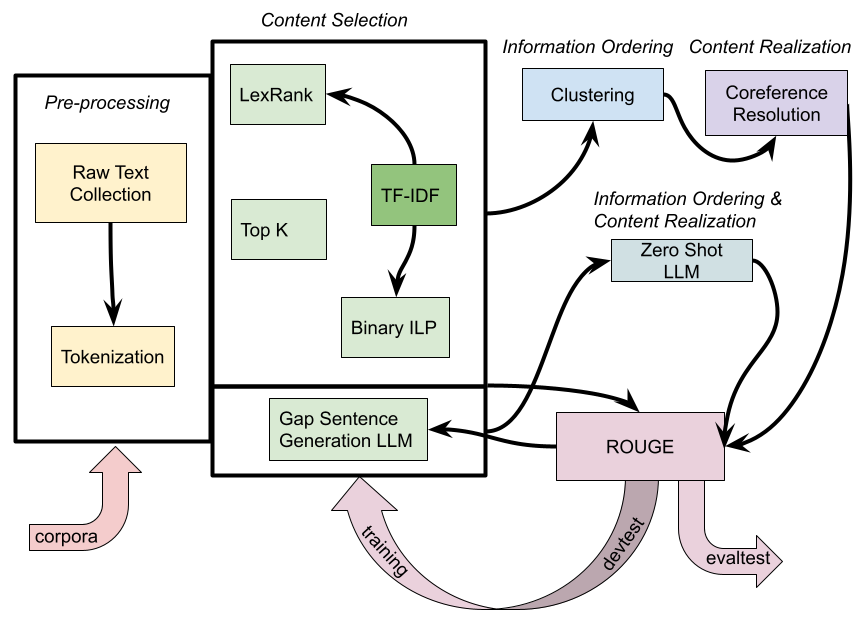
\includegraphics[scale=0.24]{D5_ System Architecture.png}
    \caption{The base system architecture from preprocessing the data to content realization}
    \label{SystemArchitecture}
\end{figure}


\section{Approach}

\subsection{Data Pre-processing}

\subsubsection{Accessing Input Data}

We used the data from the TAC 2009 \cite{tac20009}, 2010 \cite{tac2010}, 2011 \cite{tac2011} Shared Task data. TAC 2009 was used for training, TAC 2010 was use for testing, and TAC 2011 was used for validation. To process the given XML files to retrieve the set of document names in docSetA, we used xml.etree.ElementTree. We then figured out which corpus data path matched each document in docSetA.

In order to read in these AQUAINT and AQUIANT2 files that are organized differently, we used lxml.etree as this can parse non-XML compliant files. We found there are three different organization methods that were used, and we made sure to process each kind uniquely. From these files, we parsed the headline, time, and raw text paragraphs.

\subsubsection{Tokenization}

 After getting the raw text, we used NLTK \cite{nltk} for text tokenization. Specifically, we used the English model tokenizer (\texttt{tokenizers/punkt/english.pickle}). We first tokenize the document on sentence level, and then for each tokenized sentence, we ran a word tokenizer. This gave us a list of sentences, where each sentence contains tokenized words. 

\subsubsection{Sentence Embeddings}\label{sentence_embeddings}
We wanted to investigate whether semantic information can improve the performance of various algorithms used to generate summaries. We compared the performance of the LexRank and topic clustering algorithms by utilizing TF-IDF, Word2Vec \cite{mikolov2013-word2vec}, and DistilBERT \cite{Sanh2019DistilBERTAD} to generate document vectors. For the pretrained word2vec model, we used the continuous bag of words (CBOW) model trained on the Google News corpus. 

Creating vectors from each document involve different pooling methods. The TF-IDF vector was constructed by using either calculating TF-IDF for each document, with IDF values obtain either from the document set or data set. IDF values can also be derived from the training set in order to upweight uncommon words and downweight common ones. Word2vec vectors were created by averaging each word vector (obtained from the pretrained model). DistilBERT vectors were created by obtaining the final hidden states of the pretrained model, and averaging these final states.

\subsection{Content Selection}

\subsubsection{Baseline: Lead $K$}

    For our baseline we implemented taking the first $k$ sentences of the first document in the docset. If the first sentence is too long (over 100 words), we keep skipping the first few sentences until we find one sentence less than 100 words. Then, we continue adding more sentences one by one until the next sentence makes the summary over 100 words. This means possibly we could end up with a one sentence summary if the proceeding sentence already makes it over 100 words.

\subsubsection{TF-IDF}\label{content_selection_tf_idf}

    To obtain the importance of an n-gram in a given document set, we used the term-frequency, inverse document frequency (\textbf{tf $\cdot$ idf}) metric. To calculate, we used a few different formulas with different parameters. The parameters were as follows:

    \begin{itemize}
       
        \item N-gram: Whether to treat each term as a unigram, bigram, or trigram. Padding was incorporated here for both start of sentence and end of sentence tokens, using nltk.util.ngrams.

        \item Eliminate\_punctuation: Whether to include punctuation or not.

        \item Casing: Whether to lowercase all letters, or maintain original capitalization

        \item log: Whether to use logged equations or not (see equations in section \ref{content_selection_tf_idf})

        \begin{itemize}

            \item log\_base: If logged equations are used, what base to use

        \end{itemize}

        \item smoothing: Whether or not to smooth TF and IDF by adding a small value to word counts

        \begin{itemize}

            \item tf\_delta: Add a small value $\delta_1$ to word counts when calculating TF (if smoothing)
    
            \item idf\_delta: Add a small value $\delta_2$ to word counts when calculating IDF (if smoothing)

        \end{itemize}
    \end{itemize}
    One difference than normal tf-idf is that we used tf at a different level of document than idf. For LexRank we used a sentence level document, while allowing the idf to span over the entire data set. For ILP, we used a docset level document, while allowing the idf to span over the entire data set. This will help to make frequent words insignificant and help located the more important words for the sentence or document set.
 
    Using the logarithmically scaled, add $\delta_1$ smoothed tf, and we used an add $\delta_2$ smoothed idf to weight each term in the document set \citep{seki_2003}.

    Given all the training data $D$ with $N$ documents, an n-gram $t$, and a document set $d\subseteq D$, we calculated the logged term-frequency, inverse document frequency as follows: \\

    First , we let:
    \begin{align}
        f_{t,d} &= \mathrm{count}(t) \; \mathrm{for} \: t\in d \\
        n_t &= \vert \{d\mid t\in d, d\in D\}\vert
    \end{align}        

    If logged, we calculate as follows:    
    \begin{align}
        \mathrm{tf}\cdot \mathrm{idf}(t,d,D) 
            &= \mathrm{tf}(t,d)\cdot \mathrm{idf}(t,d,D) \\
        \mathrm{tf}(t,d) 
            &= \log(\delta_1 + f_{t,d})\\
        \mathrm{idf}(t,D) 
            &= \delta_2 + \log\left(\dfrac{N}{\delta_2 + n_{t}}\right)
    \end{align}
    
    If not logged, we calculate as follows:
        \begin{align}
            \mathrm{tf}\cdot \mathrm{idf}(t,d,D)
                &= \mathrm{tf}(t,d)\cdot \mathrm{idf}(t,d,D) \\
                \mathrm{tf}(t,d)
                &= \delta_1 + f_{t,d}\\
             \mathrm{idf}(t,D) 
                &= \delta_2 + \dfrac{N}{\delta_2 + n_{t}} 
        \end{align}

    If not smoothed, $\delta_1$ and $\delta_2$ effectively become $0$.

\subsubsection{Binary Linear Programming}
Previous studies such as \citet{Gillick_2008_ILP} and \citet{luo_liu_liu_litman_2018} have treated content selection as an integer linear programming (ILP) task. For this method of content selection, we also treat it as such. As with \citet{Gillick_2008_ILP} and \citet{luo_liu_liu_litman_2018}, we also used n-grams for ``concepts", specifically unigrams, bigrams, and trigrams (exclusively). Unlike \citet{luo_liu_liu_litman_2018} who used \textit{term-frequency} for their concept weights, and \citet{Gillick_2008_ILP} who used \textit{document frequency} for their concept weights, we combined the two weighting methods and used the \textit{tf-idf} of n-grams as calculated in section \ref{content_selection_tf_idf}. For the formulation of the ILP, we used the objective function, constraints, and binary variables as proposed in \citet{Gillick_2008_ILP}. 

For notation, we take a bag of sentences and bag of concepts approach. We call the given set of sentences $Y$ which constitute the given document set, and the set of concepts $Z$ which also constitute the given document set. We let the decision variable $y_j$ correspond to sentence $s_j\in Y$ and we use the decision variable $z_i$ correspond to concept $c_i\in Z$. We also let $y_j$ and $z_i$ be indicator functions, indicating whether to include or exclude a sentence $s_j$ and concept $c_i$ respectively from the summary, and thus $y_j$ and $z_i$ can only take on values of $0$ or $1$. 

We use $A_{i,j}$ to denote the indicator function $\mathds{1}_{z_i\subseteq y_j}$, i.e. $A_{i,j}$ = 1. If concept $z_i$ appears in sentence $y_j$, we give a value of 0. Otherwise. We use the weight $w_i\in\mathbb R$ where weight $w_i$ is the corresponding weight for ''concept'' $z_i$. We also have a maximum term summary length $L$. If we have $N$ sentences in the optimal summary, and $M$ sentences total in the document set, we can then formulate the optimization problem as follows:
\begin{align}
    \text{maxmimize}_{y,z} \ \ &\mathlarger\sum_{c_i\in Z} w_iz_i \label{ilp_objective} \\
    \text{Subject to} \ \ & \sum_{j=1}^M A_{i,j} y_j \geq z_i,\:\forall c_i\in Z  
    \label{ilp_concepts_selected} \\
    & A_{i,j}y_j \leq z_i, \: \forall c_i, s_j\in Z\times Y\label{ilp_all_concepts_included} \\
    & \sum_{j=1}^N l_jy_j \geq L \label{ilp_sent_length_constraint} \\
    & y_j\in \{0, 1\}, \ z_i\in \{0, 1\} \label{ilp_integer_constraint}
\end{align}

We see that Eq. (\ref{ilp_objective}) is the objective function where we are trying to maximize the total weight of the concepts chosen for the summary in an attempt to extract the most important concepts in a document set. 
Eq. (\ref{ilp_concepts_selected}) ensures that a concept is included in the optimal summary if and only if there is a sentence that is selected for the optimal summary that contains said concept.
Eq. (\ref{ilp_all_concepts_included}) ensures that all concepts in sentence $y_j$ are included if $y_j$ is included in the optimal summary. Eq. (\ref{ilp_sent_length_constraint}) ensures that the given summary remains under the maximum sentence length $L$. Eq. (\ref{ilp_integer_constraint}) ensures that the decision variables for sentences $y_j$ and concepts $z_i$ act as indicator functions. 
For each "concept'' $z_i$, we tested unigrams, bigrams, and trigrams. For the corresponding weight $w_i$ for each concept, we used the tf-idf score of the unigram, bigram, or trigram $z_i$ (exclusive) as calculated in section \ref{content_selection_tf_idf}.

Although there is no explicit redundancy checker, we see that implicitly, redundancy is kept to a minimum because of the formulation of the ILP problem--each concept weight will be included in objective function only once.

\subsubsection{LexRank}

The LexRank algorithm treats each sentence as a document. It compares sentence vectors to construct a weighted graph of the relationships between sentences in a document set. \citet{lexrank} obtains sentence vectors using TF-IDF (without smoothing); however, sentence vectors can be obtained using a number of methods (see \ref{sentence_embeddings}). We found the best performing vectors to be TF-IDF vectors with the IDF values taken from the evaluation dataset and training dataset, +1 smoothing for unseen terms for IDF, and ignoring punctuation tokens.

Sentences that are compared to one another are related to one another using the cosine similarity measure of their vector representations. For vector representation of sentences $\Vec{s_i}$ and $\Vec{s_j}$: 
\begin{align} 
    sim&(\Vec{s_i},\Vec{s_j}) = \frac{\Vec{s_i} \cdot \Vec{s_j}}{||\Vec{s_i}||_2 \times ||\Vec{s_j}||_2} \label{cosine similarity measure}
\end{align} \normalsize

\noindent A similarity matrix can then be constructed by calculating similarity scores across all sentences in the document. Unlike \citet{lexrank}, we do not calculate the similarity between instances of the same sentence, since we found 1 to be a relatively similarity high score. We believe the decline in performance might pertain to lowering other similarity scores to other sentences after the adjacency matrix's rows are normalized.

Using this similarity measure, we created a similarity matrix between sentences in the document, which also functioned as a weighted graph. Per \citet{lexrank}, values with low similarities scores and self-connections are set to zero. After perfoming row normalization, The matrix satisfies the properties of a stochastic matrix, allowing us to use the power method to estimate the eigenvalue of the matrix. We initialize the centrality vector as $\bm{p}=\frac{1}{N}\bm{p}$, where $N$ is the number of documents. We then apply the following update to  $\bm{p}$: \begin{align} 
    \bm{p} = [d\bm{U}+(1-d)\bm{B}]^T\bm{p}
\end{align}

\noindent where $\bm{U}$ is a square matrix of size $[N \times N]$ with values equal to $1/N$ and $\bm{B}$ is the adjacency matrix of the graph. 

Experiments were conducted to investigate whether LexRank performed best with TF-IDF, Word2vec, or DistilBERT vectors. A comparison table can be found in Appendix \ref{appendixtable}.

\subsubsection{Gap sentence generation} \label{GSG}
We used the gap sentence generation method introduced in \citet{pegasus}. Based on the finding when \citeauthor{pegasus} were training the Pegasus based model, we will selecting the top m sentences as gap sentences without replacement from a document based on importance score. The importance score is calculated based on the ROUGE score one sentence gets comparing to the remaining sentences in one document as in Algorithm ~\ref{alg:GSG}.

\begin{algorithm}[H]
\caption{Independent sentence selection}\label{alg:GSG}
\begin{algorithmic}[1]
\State $ \textit{D} := \{x_i\}_n \gets \text{sentences in whole docset}$
\State $ \textit{S} := \emptyset$
\State $ \textit{I} \gets \text{list contains index from 0 to n}$
\For{$j \gets 1 \text{ to } n$} 
\State $ s_i := \textit{ROUGE}(x_i, D \setminus \{x_i\}) $
\State $ S := S \cup \{s_i\} $
\EndFor
\State $ I := sort(I) \text{ Based on the value in S}$
\end{algorithmic}
\end{algorithm}

To improve the system, when we are processing the training data, we calculate the ROUGE score based on the average ROUGE score when comparing the selected sentence with each of the gold summary. We only calculate the ROUGE score based on the rest of the documents when we are processing the test and validation data.

We only mask the top thirty percent of the sentences as \citeauthor{pegasus} finds out achieves relatively high performance without sacrifice training efficiency.

\subsection{Information Ordering}

\subsubsection{Topic Clustering}

This algorithm tries to order topics in the order that they are most likely to appear in a document. The intuition being that similar sentences form topics, and topics must be ordered in the original documents in a cohesive manner. This algorithm tries to recreate this cohesive topic order. This algorithm is heavily modified from the 'Augmented Ordering Algorithm' presented in \citet{barzilay_2002}. Barzilay groups similar themes from different documents into blocks, and then orders the blocks by timestamp. However, in our algorithm, we instead put all of the documents together and consider it one document, clustering similar sentences/topics of information into themes. There are no senses of block here as discussed in \citet{barzilay_2002}.

Similarity between sentences is determined by the similarity of sentence embeddings. To group topics, we group similar sentences over a whole document set. We calculate sentence as calculated in section \ref{sentence_embeddings} using TFIDF embeddings for each word in a sentence. We have chosen between TFIDF, Word2Vec, and DistilBERT as a hyperparemeter for sentence embeddings. Please see Tables \ref{clustering_mean} and \ref{clustering_median} for an error analysis between them.

We then use sentence embeddings to create topic clusters to group similar sentences. To group sentences, we used K-means clustering using \texttt{sklearn.cluster.KMeans}. 

To order topic clusters, we used the 'fractional ordering' of the sentences, namely, let $d$ be a document with length $n$, then the fractional ordering $f$ of sentence $s_i$ at position $i$ in $d$ is:
\begin{align}
    f(s_i, d) = \dfrac{i}{n}
\end{align}

For example, the first sentence in the given document is always $\dfrac{1}{n}$, the second $\dfrac{2}{n}$, etc. We divide by the number of sentences in the document to try to normalize both short and long documents. 

We then ordered each topic cluster $t_k$ with $m$ sentences by their respective median fractional ordering, namely, for each sentence $j$ in the given topic, the median fractional ordering $f_{med}$ is found by sorting all the fractional orderings for each sentence, and using the one in the middle.

Using average (see below) versus median fractional ordering was another hyperparameter we chose from\footnote{Please see Table \ref{clustering_mean} and Table \ref{clustering_median} in for an error analysis between them.}

The average fractional ordering $f_{avg}$ is:
\begin{align}
    f_{avg}(t_k) = \dfrac{\sum_{j} f(s_j, d)}{m}
\end{align}

We then order the sentences in the given summary based on which topic cluster they appear in and the fractional ordering of that topic. In other words, if $f_{med}(t_k) < f_{med}(t_k')$, then any sentence that appeared in the summary and in topic cluster $t_k$ would appear before all the sentences that appeared in the summary and in topic cluster $t_k'$. 

 It is possible that multiple sentences appear in the given summary and the same topic cluster. In this case, we order the sentences by their own fractional ordering. In other words, for sentence $i$ and sentence $j$ in documents $d$ and $d'$ respectively, if $f(i, d) < f(j, d')$ we put sentence $i$ before sentence $j$ in the ordered summary.

% to do if we have time
%  \begin{algorithm}[H]
% \caption{Topic Clustering}\label{alg:clustering}
% \begin{algorithmic}[1]
%     \State $S := \{s_i\}_n \gets \text{n sentences in document set}$
%     \State $S^* := \{s^*_k\}_m \gets \text{m sentences in summary}$
%     \State $e := \emptyset$
%     \For{$i\gets 1 \text{ to } n$}
%         \State $e_i \gets \text{embedding representation of } s_i$
%         \State add $e_i$ to $e$
%     \EndFor
%     \State Cluster embeddings $e$ into $t$ themes $\{t_j\}_t$

%     \For{$j \gets 1 \text{ to } t$}
%         \State $f_{j} \gets f_{med}(t_j)$ or $f_{mean}(t_j)$
%     \EndFor
%     \State Order themes by $f_j$
%     \State $S^* = \emptyset$
%     \For{$k\gets 1 \text{ to } m$}
%         \State $s^*_k \gets \text{sentence } k \text{ in summary}$

%         \For{$j\gets 1 \text{ to } t$}
%             \If{$s^*_k\in t_j$}
%                 \State $f_{s^*_k} := f_j$
%             \EndIf
%         \EndFor
%     \EndFor
    
    
% \State $ \textit{D} := \{x_i\}_n \gets \text{sentences in all}\textit{document}$
% \State $ \textit{S} := \emptyset$
% \State $ \textit{I} \gets \text{list contains index from 0 to n}$
% \For{$j \gets 1 \text{ to } n$} 
% \State $ s_i := \textit{rouge}(x_i, D \setminus \{x_i\}) $
% \State $ S := S \cup \{s_i\} $
% \EndFor
% \State $ I := sort(I) \text{ Based on the value in S}$
% \end{algorithmic}
% \end{algorithm}

\subsubsection{Seq2Seq language model}

We fin-tuned a sequance to sequance language model based on the implementation of Reorder-BART (RE-BART) by \citeauthor{rebart}.  RE-BART is a fine-tuned model based on BART by to identify a coherent order for a given set of shuffled sentences. We shuffle the sentences of each input document set based on the Gap sentence generation content selection method without masking. We mark the index of the sentences at the beginning of each sentences. The model takes the sets of shuffled sentences with sentence-specific markers as input and generates a sequence of position markers of the sentences in the ordered text. We trained the model using Huggingface transformer library \citet{transformers}. We trained the model using the PyTorch framework with a NVIDIA A100 GPU. We trained the model with batch size of 4 and epoch of 24. 

\subsubsection{ROUGE score ranking}
Due to the input size limitation for the majority of the language model, we have to truncate the input text to 1024 tokens. After we mask the important sentence, we then use the ROUGE score ranking calculated for the gap sentence generation to discard sentences that are ranked in the low thirty percent. We keep the ordering of the remainder of the sentences. Discarding unimportant sentences based on ROUGE score helps including more important sentences from multiple documents. When discarding, we calculate the token length for each added sentences and stop when adding additional sentence will cause the token size to exceed 1024 tokens. This make sure we have full sentences for the input sequence.

To improve the system, we experiment on multiple parameters, such as what the percentage of the sentences should we discard. We also calculate the ROUGE score ranking based on either the average score based on the gold summary or based on all of the remaining sentences in all provided documents. 


\subsection{Content Realization}

\subsubsection{NP Rewrite}
We developed an entity replacement method inspired by the noun phrase rewriting method for multi-document summarization method described in \citet{siddharthan-etal-2011-information}. We take each document set being analyzed and cluster spans into categories denoting  the same entity. We accomplish this task using an experimental module spaCy \cite{spacy}. The module obtains token embeddings from RoBERTa and then obtains a score for embedding pairs before passing the score to a linear classifier (along with other features) to determine whether the spans refer to the same entity \cite{spacycoref}. Because the number of spans is $O(n^2)$, calculating each potential coreference is computationally expensive, so the spaCy implementation prunes the number of spans to compare before obtain the results from the linear classifier, adapting an algorithm described in \cite{dobrovolskii-2021-word}.

% replace indices on the sentences, and say NP in the set of clusters (use set notification to describe the clusters {c|c in ,,,})

We adapted our NP replacement algorithm from \citet{siddharthan-etal-2011-information}. We use our ILP and LexRank methods to extract the sentences with the highest weights. We also obtain coreference clusters for the entire document set (concatenating the documents) using spaCy's module described above. We apply the model to the concatenated document to minimize the number of clusters with the same or similar spans. Then, using, spaCy base module \cite{spacy}, we obtain the noun phrases contained in the highest-ranked sentence. For each NP in the highest-ranked sentence, we examine its coreferring NPs in the document set and replace it with the longest pre-modifidying NP. We use a rough heuristic to extract the longest pre-modified by discard all text followed by appositives, since those formed the bulk of the post-modifiers described in \citet{siddharthan-etal-2011-information}. If the longest pre-modifidying NP is the same length as the NP itself, we look for the longest post-modifying phrase. The cluster containing the longest pre-modifying NP is indexed. For all future NPs and sentences, if $NP_i \in s_j$ is contained in a seen cluster $c_k$, then the shortest non-pronominal NP is chosen to replace it. If the $NP_i \in s_j$ is not contained in a seen cluster $c_k$, it is replaced with the longest modifying phrase. This intuition was drawn from the observations of \citet{siddharthan-etal-2011-information}, about keeping NPs of previously seen referents terse and expanding upon unseen referents.

In addition, added a few small rules to ensure a readable summary. We did not replace the pronoun "I" in the context of quotes. We also did not replace proper nouns with noun phrases that did not have word overlaps with the original expression. We also made sure that, if both the replacement and the original NPs contained pronouns, those pronouns must agree in grammatical case (to avoid ``we'' being replaced with ``our'').

\subsubsection{Redundancy Removal}\label{sec:redundancy}

After obtaining a ranked order of extracted sentences, we experimented with removing redundant sentences using the Jaccard similarity measure. Sentences with the top-$k$ values in ranking are extracted and added to the summary text until the summary reaches the maximum length. To avoid repeated information, we use the Jaccard similarity measure (provided by NLTK) to calculate each sentence's similarity to sentences already included in the bibliography \cite{bird-loper-2004-nltk}. To calculate Jaccard similarity for sentences, let $J$ denote the similarity function, $w$ denote a word and $s_i, s_j$ denote two sentences.
\begin{align} 
    J(s_i, s_j) = \frac{|\{w|w\in s_j\} \cap \{w|w\in s_i\}|}{|\{w|w\in s_i\} \cup \{w|w\in s_j\}|}
\end{align}

\noindent Additionally, sentences that are too long are discarded. We discard long sentences because we believe these sentences are likely to be too information-dense to be useful for constructing a summary. We also discard sentences that were a part of a quotation that was cut off by the tokenizer since we currently have no way of evaluating the importance of the sentence combine with its reconstructed context. The redundancy removal method was employed by the LexRank algorithm, but not by others. The algorithm is described in pseudo-code in algorithm \ref{alg:redundancy}. 

\begin{algorithm}[ht]
\caption{Redundancy removal algorithm}
\small
\hspace*{\algorithmicindent} \textbf{Input:} $top_k$, $max_w$, $min\_jaccard$\\
\hspace*{\algorithmicindent} \textbf{Output:} Summary string
\begin{algorithmic}[1]
\State $\mathrm{Array} \ S \gets \mathrm{LexRank} (doc)$
\State $\mathrm{Array} \ SeenSentences$
\State $\mathrm{String} \ Results$
\State $\mathrm{Int} \ Length \gets 0$
\State $\mathrm{Int} \ i \gets 0$
\While{$i \leq top_k$ or $i \leq \textrm{Len}(S)$}
    \State $\mathrm{Bool} \ CheckJaccard \gets True$
    \For{$j \gets 1 \ \mathrm{to} \ \mathrm{len}(SeenSentences)$}
    \If{$D_{j}(S[i], S[j]) \geq min\_jaccard$}
    \State $CheckJaccard \gets False$ 
    \EndIf
    \EndFor
    \If{$CheckJaccard$ is $False$}
        \State $i \gets i+1$
    \ElsIf{$\mathrm{len}(S[i]) + Length > max_w$}
        \State $i \gets i+1$
    \Else
        \State $w \gets w + \mathrm{len} (S[i])$
        \State $Results \gets Results \oplus S[i]$
        \State $SeenSentences \oplus S[i]$
        \State $Length \gets \mathrm{len}(S[i]) + Length$
        \State $i \gets i+1$
    \EndIf
\EndWhile 
\end{algorithmic} \label{alg:redundancy}
\end{algorithm} 
\normalsize

\subsubsection{Sequence to Sequence language model}
We fin-tuned "google/pegasus-large" and "google/pegasus-cnn\char`_dailymail" to generate the summary based on preprocessed input data discussed in Section \ref{alg:GSG}. We utilized the Huggingface's transformers library for the experiment. The experiments are conducted in PyTorch framework using NVIDIA Tesla A100 GPU. We trained on the training data and use the devtest data to select the best model based on the ROUGE 1 score of output summary based on devtest data.

\section{Results}

Table \ref{tab:rouge_devtest} and \ref{tab:rouge_evaltest} show the performance of the selected summarization methods on the TAC 2010 (devtest) and TAC 2011 (evaltest) datasets.\footnote{The scores in these tables used the official ROUGE Perl script which, from our observations, tends to have lower scores than the Python modules. We believe this is due to the fact that the Perl script performs bootstrap oversampling as opposed to the Python module.} The best ROUGE 1 numbers of each dataset are bolded. Our experiments show that the Binary ILP achieves the highest ROUGE 1 score based on the evaltest dataset.

The Binary ILP scores use a system that included Binary ILP, topic clustering, and NP-replace. The LexRank scores reflect a system that included LexRank, topic clustering, and redundancy removal.

\begin{table}[H]
    \caption{ROUGE recall scores on \textbf{devtest} files}
    \centering
    \begin{tabular}{c|c|c}
        \hline 
         & ROUGE1 & ROUGE2 \\
         \hline
         Best of TAC 2011 & - &  9.574\\
         Binary ILP & 23.616 & 5.919 \\
         LexRank & \textbf{24.959} & 6.936\\
          GSG LLM & 19.162 & 5.129 \\
          Baseline Lead K & 17.122 & 4.936 \\
         \hline
    \end{tabular}
    \label{tab:rouge_devtest}
\end{table}

\begin{table}[H]
    \caption{ROUGE recall scores on \textbf{evaltest} files}
    \centering
    \begin{tabular}{c|c|c}
        \hline 
         & ROUGE1 & ROUGE2 \\
         \hline
         Best of TAC 2011 & - & 13.440 \\
         Binary ILP & 27.700 & 7.972 \\
         LexRank &  \textbf{29.328} & 9.217\\
          GSG LLM & 21.396 & 5.723 \\
          Baseline Lead K & 23.030 & 7.585 \\
         \hline
    \end{tabular}
    \label{tab:rouge_evaltest}
\end{table}

\subsection{Integer Linear Programming}
To find the best combination of hyper-parameters, we ran a manual coordinate descent on our hyper-parameters. For each set of experiments, we changed one hyper-parameter at a time declaring the best value for each hyper-parameter only after the conclusion of each set of experiments. We then would keep this best value for the subsequent experiments until we had run experiments for every hyper-parameter.

With the above method, we found that the best combination of hyper-parameters to pass in to our calculation of tf-idf was to use calculate tf-idf for unigrams, using a logged tf-idf with $\delta_{1}$ close to 0 (in our case $\delta_{1} = 0.01$), a $\delta_{2}$ close to $1$ (our best case uses $\delta_{2} = 0.7$). We also found that eliminating punctuation and lowercasing all tokens yielded the best results. We also found that removing sentences with less than around 25 tokens\footnote{We count tokens after begin tokenized by \texttt{nltk.word\_tokenize}} yielded the best ROUGE scores. 

\subsection{Large Language Model}

For our experiment for finetuning the PEGASUS model, we tested different combinations of the training arguments, such as different epoch and difference batch sizes. Table \ref{tab:rouge-LLM} listed all parameter changes we make for out experiment. ROUGE-on stands for calculating the ROUGE score of a selected sentence from a document, either with the other sentences in that document (single) or with the other sentences in all the documents in a docset (multi). We also experiment on different epoch. Discard stands for the percentage of sentences we selected to discard when generating the input. For example, if we change the ROUGE-on parameters to multi, then choosing 50\% discard rate means that we will discard the bottom 50\% of the sentences in all of the documents in a docset based on how high the ROUGE score is.
Combine masking stands for whether or not we concatenate the gap-sentences into a single mask token. The result shows that when we calculate the ROUGE score of the selected sentence with the rest of the sentences in all documents in one docset, discard bottom 50\% of the sentences, and combine multiple masked sentences into a single mask token achieve the highest ROUGE 1 and ROUGE 2 score for the devtest data. We also experiments with both "google/pegasus-large" and "google/pegasus-cnn\_dailymail" checkpoints for the PEGASUS model. We find out that the news-summarzation focused "google/pegasus-cnn\_dailymail" performs better than "google/pegasus-large", which trained on more datasets than "google/pegasus-cnn\_dailymail.

\begin{table*}[ht]
    \centering
    \begin{tabular}{c|c|c|c|c|c|c}
        \hline 
         model & ROUGE-on & epoch & Discard & \multicolumn{1}{|p{1.5cm}|}{\centering Combine\\Masking} & ROUGE1 & ROUGE2 \\
         \hline
         pegasus-large & single & 6 & 50\% & True & 0.21037 & 0.06214 \\
         pegasus-large & multi & 12 & 50\% & True & 0.26419 & 0.05367\\
         \rowcolor{green!30} pegasus-large & multi & 24 & 50\% & True & 0.28415 & 0.06464\\
         \rowcolor{yellow!30} pegasus-cnn\_dailymail & multi & 24 & 50\% & True & 0.31355 & 0.08191\\
         pegasus-large & multi & 12 &30\% & True & 0.24330 & 0.04773\\
         pegasus-large & multi & 12 & 30\% & False & 0.24263 & 0.05343\\
         \hline
    \end{tabular}
    \caption{Large langauge model ROUGE Recall Scores with different parameters}
    \label{tab:rouge-LLM}
\end{table*}

We also experiment on the zero-shot learning method for information ordering using the BART model. The result, however, is disappointing. The model we trained for our experiment failed to generate a sequence of position makers as output. Instead, the model directly generates the ordered text as the output where each sentences are compressed and no longer contain the same level of information compare to the original sentences. We tried to investigate the cause of the issue by reducing input sizes, and increase training data coverage by including all of the sentences from training, testing, and validation data into groups of six sentences. We tried to tweak other parameters such as increasing the training epoch from 8 to 24. However, none of the above methods leads to having the generated output from the fine-tuned model produces sentence indexes, and we choose not to move forward with this information ordering method.

\subsection{Topic Clustering}

To run K-means clustering, we used 8 clusters, and the following parameters for \texttt{sklearn.clusters.KMeans}\footnote{These are the default parameters provided by \texttt{sklearn.cluster.KMeans}, and we did not test our topic clustering algorithm on other hyper-parameters.}:

\begin{verbatim}
    kmeans = KMeans(
        n_clusters=8, init='k-means++', 
        n_init=10, max_iter=300, 
        tol=0.0001, verbose=0, 
        random_state=None, copy_x=True, 
        algorithm='lloyd')
\end{verbatim}

We also chose to use the median fractional ordering (rather than the mean fractional ordering) and \textit{tf-idf} vector embeddings (as opposed to DistilBert or Word2Vec vector embeddings) to order the sentences in the summary.

\subsection{Content Realization}

The addition of the NP-replace algorithm did not significantly alter the results of the ROUGE scores (see Section \ref{section::ablation} below). Upon visually examining the data, the algorithm does not seem to make a significant impact on the quality of the summaries. It's successes are certainly diminished by the frequency of its failures. Additionally, we suspect that because the unsupervised methods seem to favor longer, more descriptive sentences, replacing NPs is should not be considered to be a priority.

On the other hand, detecting redundant sentences and excluding them from the final summary does seem to be more impactful on the resulting ROUGE score. We performed an ablation study to better understand its impact which is described in more detail below.

\subsection{Ablation Studies on LexRank}\label{section::ablation}

An ablation study was performed on the LexRank algorithm in combination with the redundancy removal algorithm (see \ref{sec:redundancy}). We compared the systems that naively chose the top ranked sentences until the maximum number of summary tokens is reached, a system that checks for similarity with existing sentences in the summary to eliminate redundancy, and a system that both checks for redundancy and performs NP-replacement. A list of ROUGE scores for these systems are found in table \ref{tab:ablation}. This finding is also surprising given LexRank's reliance on similarity scores to generate the graph representation of a document.

\begin{table}[H]
\centering
\begin{tabular}{|p{4cm}|p{1cm}|p{1cm}|}
  \hline
    System  & R-1 & R-2 \\ \hline
    LexRank & 24.215 & 7.201 \\
    LexRank $+$ Redundancy & \textbf{24.959} & \textbf{7.437} \\
    LexRank $+$ Redundancy $+$ NP-Replace & 24.552 & 7.211 \\ \hline

\end{tabular} \caption{LexRank Ablation ROUGE Scores (Recall)}
\label{tab:ablation}
\end{table}

Interestingly, the neither the redundancy removal algorithm nor NP-replace significantly impact the performance of the algorithm (as measured by ROUGE scores). Visual examination indicates that between 3-6 sentences are selected for a typical summary and that it is uncommon for sentences to be similar. We speculate that either the summaries are too short for redundancy removal to have an effect on ROUGE scores or the minimum Jaccard distance chosen for the experiment (0.7) is too low (however, visual examination did not reveal redundancy to be a pervasive issue).

\subsection{Error analyses}

\subsubsection{Error Analysis of \textit{devtest} data}

We perform a casual error analysis for the summaries based on \textbf{devtest} docset D1006, which are shown in Table \ref{tab:error_analysis_devtest}.

The improved Binary ILP method makes leaps in achieving a better summary from D3. The old summary seemed to give important facts concerning the FDA and withdrawing Vioxx, but seemed to have a lot of more "unimportant facts" that didn't help the reader get a clear idea of what the article is about. An example of this is mentioning about rewriting abstract conclusions, and the amount of teleconferences that were gone to. The improved summary gives a clear picture of the latest update on Vioxx and the new findings of effects its gives. Comparing the output of D4 and D5, there does not seem to be a difference. This may be because the new hyperparameters from clustering did not effect the sentence ordering here, and content realization did not find anything to use co-reference resolution on.

The improved LexRank method no longer produce unncessary information such as website address. The improved method successfully mention Vioxx, where the old method did not. However, the improved method still failed to catch one of the core story point, that Vioxx is recalled by the company. The improved method does capture that Vioxx has potential cardiovascular risks. Interestingly, the using TF-IDF vectors resulted in better performance than using word2vec or DistilBERT sentence vectors. A comparison is shown in Table \ref{tab:lexrank_expt} in Appendix B.

The summary produced by the improved GSG LLM method provides more specific details than the previous system iteration. For example, it mentions that Vioxx was used by 20 million Americans, was Merck’s top-selling product, and that Merck had spent \$195 million to promote it. It also mentions that the FDA had been concerned about the drug’s cardiovascular risks since at least 2000 but did not issue a warning until 2004. These details provide more context and a better understanding of the situation. Another improvement is that it provides a clearer timeline of events. It mentions that Vioxx was approved in 1999, that the FDA had been concerned about its cardiovascular risks since at least 2000, and that the drug was recalled in 2004. This helps the reader understand the sequence of events and the time frame in which they occurred. Compared to the gold summary, however, the improved system still lacks certian information. For example, the improved GSG LLM method generated summary lacks information about the specific clinical trial that led to the recall of Vioxx. The gold summary mentions that the clinical trial was for the use of Vioxx in colon cancer and that it showed unacceptable rates of stroke and heart attack. The generated summary also does not mention that Vioxx was a COX inhibitor, which was safer for the digestive tracts of arthritis patients. Additionally, the gold summary mentions concerns about drug manufacturers’ advertising and the FDA’s role in ensuring the safety of drugs on the market, which is not mentioned in the generated summary.

The summary produced by the baseline mentions a small amount of important details such withdraw the specific drug and how many people used it. But fails to mention many other important details mentioned in the gold standard and by the other methods.

\subsubsection{Error Analysis of \textit{evaltest} data}
We perform a casual error analysis for the summaries based on \textbf{evaltest} docset D1105, which are shown in Table \ref{tab:error_analysis_evaltest}.

For the ILP method, it mentions most of the details in the gold standard summary. It does miss the exact date of the crash, and how many killed/ possible survivors. It also missed the detail on the unknown cause of the crash, but does mention about the stormy weather.

For the GSG LLM method, the generated summary correctly states that an Adam Air Boeing 737-400 plane with 102 people on board crashed in a mountainous area near the town of Polewali, on its way from Surabaya to Manado. It also correctly states the casualty count of the crash. These are some of the main points of the gold text that the generated summary accurately captures. However, the generated summary lacks additional details such as the weather condition might be a factor of the crash, and there were three Americans on board. Lastly, the generated summary introduces new information about the Indonesian Navy sending planes to carry the bodies of its members, which is not mentioned in the gold text. Overall, the generated summary captures some of the main points of the gold text, but also contains errors and omissions.

The baseline seems to mention mostly about a different event, but mentions the main event the gold standard summary is concerned about in the last sentence. This may be because the first article in the docset mentions about both the events in the first few lines.

\subsubsection{Error analysis of Information Ordering}

Although the correct ordering of a summary is most definitely subjective, we feel that ordering by median fractional ordering, as well as using \textit{tf-idf} vector embeddings produced the best, most cohesive summaries.

In both table \ref{clustering_mean} and \ref{clustering_median}, we see that the summary of D1002-A using \textit{td-idf} embeddings follows a rough chronological order, namely there is a shooting (sentence 1), an accusation (sentence 2), a trial (sentence 3), and an elaboration of the trial (sentence 4). This is unlike the Word2Vec and DistilBert embeddings, which follows a timeline which is not as intuitive or cohesive, namely there is an accusation (sentence 1), an elaboration of the trial (sentence 2), etc. 

The summary order produced for D1001-A using \textit{td-idf} is less convincing in both tables \ref{clustering_mean} and \ref{clustering_median}, but it still follows a rough cohesive manner, namely there is grieving (sentence 1), then uniting and healing (sentence 2), then some moving on (sentence 3). In our opinion, sentence 4 "The school wanted..." feels out of place, it possibly be ordered between sentence 2 and 3, but it also just feels like it doesn't quite belong in this summary in general, which would be a problem with our content selection method rather than our information ordering method. 

Looking at tables \ref{clustering_mean} and \ref{clustering_median}, we can also see that looking at mean versus median, only one summary changed, namely the summary of document set D1001-A contained in the top row using \textit{tf-idf} embeddings. We therefore concluded that whether we use median or mean fractional ordering matters little. 

\subsubsection{Error analysis of Content Realization}

Examples of errors in the NP-replace algorithm can be found in table \ref{tab:error_analysis_realization}. The NP-replace algorithm is highly dependent on the performance of \texttt{}{spaCy}'s experimental coreference resolution model \cite{spacy}. Oftentimes, it clusters unrelated entities together. For instance, in the document set D1042, it associates the noun phrase ``a court martial'' with the noun phrase ``a deal'' (a bug is likely responsible for clipping the sentence). Additionally, the longest pre-modified NP isn't always the most complete description, sometimes making a sentence less readable. For instance, for document set D1010.B, the algorithm correctly marks the NP ``Suspected variant Crutzfeld-Jakob Disease'' a coreferring to the same entity as in the expression ``The fatal brain-wasting disease''. However, here the longer replacement is less descriptive than the longer one, since few readers know about Crutzfeld-Jakob Disease. Additionally, there were issues with the way \texttt{spaCy} parses noun phrases. In D1024, it parsed ``El-Shifa'' as two separate noun phrases, resulting in an awkward replacement. There were also some issues with ensuring that the grammar and punctuation matched the sentence.

\begin{table*}[ht]
\centering
\begin{tabular}{|p{1.5cm}|p{5.5cm}|p{5.5cm}|p{2cm}|}
  \hline
Doc. Set & Sentence & Replacement & Description \\
 \hline
    D1042 & Lynndie England on Monday pled guilty to charges of abusing Iraqi prisoners at the Abu Ghraib prison but told \textbf{a court martial} \underline{she} did not believe she was doing wrong when photographed holding a leash on a naked inmate. & Lynndie England on Monday pled guilty to charges of abusing Iraqi prisoners at the Abu Ghraib prison but told \textbf{the deal} \underline{she} did not believe & Coreference error $+$ bug \\ \hline
    D1002 & Through their lawyers, the officers have said \textbf{they} thought Diallo had a gun. & Through their lawyers, the officers have said \textbf{the couple} thought Diallo had a gun. & Wrong referent \\ \hline
    D1010 & \textbf{The fatal brain-wasting disease} is believed to come from eating beef products from cows struck with mad cow disease. & \textbf{Suspected variant Crutzfeld-Jakob Disease} is believed to come from eating beef products from cows struck with mad cow disease. & Longer referent is less easy to read \\ 
    \hline
    D1024 & [...] Sudan maintains \textbf{it's} a pharmaceutical plant. & [...] Sudan maintains \textbf{El-'s} a pharmaceutical plant. & Parser error \\ \hline
\end{tabular}\caption{Examples of content realization errors (devtest data)}
\label{tab:error_analysis_realization}
\end{table*}

\section{Discussion}

\begin{table*}[ht]
\centering
\caption{Generated summaries based on \textbf{devtest} docset D1006}
\begin{tabular}{|l|p{13cm}|}
  \hline
 gold & On Sept 30, Merck voluntarily recalled the pain killer Vioxx, used by almost 2 million, after clinical trials for its use in colon cancer showed unacceptable rates of stroke/heart attack. Results corroborated earlier warnings that had not resulted in recalls by the Food and Drug Administration (FDA). As a COX inhibitor, Vioxx was safer for digestive tracts, important for arthritis patients. Merck's advertising campaigns did not clearly warn about side effects. The case highlighted concerns about drug manufacturers' advertising and FDAs role in insuring safety of drugs on the market. Safety of other COX inhibitors is now a concern." \\
 \hline
ILP D5 & Merck officials said last week its latest research showed an increased risk of heart attack and other cardiovascular complications in patients who took Vioxx for at least 18 months.
Heavily advertised as an arthritis drug, Vioxx was pulled from the market last week after its maker said a study showed it doubled the risk of heart attack and stroke.
But some doctors say this group of drugs may work in a way that increases the risk of heart problems for some patients, and they point to this latest information as additional reason for concern.
 \\
 \hline
ILP D4 & Merck officials said last week its latest research showed an increased risk of heart attack and other cardiovascular complications in patients who took Vioxx for at least 18 months.
Heavily advertised as an arthritis drug, Vioxx was pulled from the market last week after its maker said a study showed it doubled the risk of heart attack and stroke.
But some doctors say this group of drugs may work in a way that increases the risk of heart problems for some patients, and they point to this latest information as additional reason for concern.
 \\
  \hline
 \multicolumn{1}{|p{1.2cm}|}{\centering LexRank \\ (D4)} & With Vioxx, researchers had been warning about the drug's possible cardiovascular risks since 2000, only a year after it was approved by the FDA . Data from a company study found then that users had four times as many heart attacks and strokes as those who used another painkiller . But the data was not definitive, and Merck, which even critics say is one of the most responsible drug companies, repeatedly reassured the medical and financial communities that Vioxx was safe.
 \\
 \hline
 \multicolumn{1}{|p{1.2cm}|}{\centering LexRank \\ (D3)} & \" That's the tragedy here . ''
 And if courts determine that Merck was negligent, the company will pay a heavy price in compensation.
 It is in the insurance industry's interest, the FDA's interest and the federal government's interest--because the federal government is a major provider of health insurance--either to require drug companies to conduct such comparative tests or to set up a neutral agency to do so.
 FDA: http: //www.fda.gov/
 \\
 \hline
\multicolumn{1}{|p{1cm}|}{\centering GSG LLM \\ (D5)} & In September 2004, Merck \& Co. recalled its arthritis drug Vioxx after a clinical trial showed it doubled the risk of heart attacks and strokes. 
 The drug had been used by 20 million Americans since its approval in 1999 and was the company's top-selling product. 
 Merck had spent \$195 million to promote Vioxx as a wonder drug for the aging baby boomers. 
 The FDA, which approved Vioxx for use, had been concerned about the drug's cardiovascular risks since at least 2000 but did not issue a warning until 2004.
 \\
 \hline
\multicolumn{1}{|p{1cm}|}{\centering GSG LLM \\ (D4)} &  Merck recalled Vioxx in September 2004 after a study showed that it doubled the risk of heart attacks and strokes in older people taking it for at least three years. 
 The drug had been approved by the FDA in 1999 for arthritis. 
 Merck had promoted Vioxx as a way to lower blood pressure and cholesterol, but the study showed that it increased the risk of heart attacks and strokes. 
 Merck's decision to withdraw Vioxx from the market raised questions about aggressive marketing of the drug before its long-term safety had been proven.
\\
\hline
\multicolumn{1}{|p{1cm}|}{\centering Baseline \\ Top K \\ (D5)} & Merck Co. said its surprise decision Thursday to withdraw the arthritis drug Vioxx--used by about 2 million people worldwide--was driven by recent evidence that the drug's adverse side effects outweighed any potential benefits.
But that wasn't really news. 
\\
  \hline
\end{tabular}
\label{tab:error_analysis_devtest}
\end{table*}
\begin{table*}[ht]
\centering
\caption{Generated summaries based on \textbf{evaltest} docset D1105}
\begin{tabular}{|l|p{13cm}|}
  \hline
 gold & Boeing 737-400 plane with 102 people on board crashed into a mountain in the West Sulawesi province of Indonesia, on Monday, January 01, 2007, killing at least 90 passengers, with 12 possible survivors. The plane was Adam Air flight KI-574, departing at 12:59 pm from Surabaya on Java bound for Manado in northeast Sulawesi. The plane crashed in a mountainous region in Polewali, west Sulawesi province. There were three Americans on board, it is not know if they survived. The cause of the crash is not known at this time but it is possible bad weather was a factor. \\
 \hline
ILP & An Indonesian lawmaker Tuesday criticised what he said was the slow deployment of search and rescue teams to a mountainous area of Sulawesi island where a plane carrying 102 people crashed.
An Indonesian passenger plane carrying 102 people disappeared in stormy weather on Monday, and rescue teams were sent to search an area where military aviation officials feared the Boeing 737-400 aircraft may have crashed.
An Adam Air Boeing 737-400 plane with 102 people on board crashed in a mountainous area near the town of Polewali late Monday on its way from Surabaya to Manado.
 \\
  \hline
 LexRank & 
 \\
 \hline
 GSG LLM & The Indonesian Navy (TNI AL) has sent two Cassa planes to carry the bodies of five of its members who were killed in a plane crash in Sulawesi late Monday. 
 An Adam Air Boeing 737-400 plane with 102 people on board crashed in a mountainous area near the town of Polewali late Monday on its way from Surabaya to Manado. 
 At least 90 people, including five TNI AL members, were killed in the crash.
 \\
 \hline
 Baseline & Indonesian President Susilo Bambang Yudhoyono said Tuesday he was deeply concerned with the crash of a passenger plane and the sinking of a ferry in the last few days that might have killed hundreds of people.
Earlier on Friday, a ferry carrying 628 people sank off the Java coast with some 400 passengers reported missing.
A Boeing 737-400 plane with 102 people onboard crashed into a mountain in the West Sulawesi province Monday, killing at least 90 people.
JAKARTA, Jan. 2 (Xinhua)
 \\
 \hline
\end{tabular}
\label{tab:error_analysis_evaltest}
\end{table*}
\begin{table*}[t]
    \centering
    \begin{tabular}{|c|p{4.3cm}|p{4.3cm}|p{4.3cm}|}
        \hline
        Docset & TF-IDF & Word2Vec & DistilBert \\
        \hline
        D1001-A & 
        \textcolor{violet}{Graham praised the Columbine community for uniting under the pain of a tragedy that could have torn it apart.}
        
        \textcolor{blue}{But Wells said he is more interested in simply trying to have fun and move beyond the tragedy that put his life on hold.}
        
        \textcolor{purple}{So many forms of community, rippling outward from Columbine High and across the planet, have come together since last week's violence that it was difficult to tell.}
        
        \textcolor{green}{The school wanted to make sure there was enough to eat since students couldn't leave campus for lunch and get back in.}
        & 
        \textcolor{purple}{So many forms of community, rippling outward from Columbine High and across the planet, have come together since last week's violence that it was difficult to tell.}
        
        \textcolor{violet}{Graham praised the Columbine community for uniting under the pain of a tragedy that could have torn it apart.}
        
        \textcolor{green}{The school wanted to make sure there was enough to eat since students couldn't leave campus for lunch and get back in.}
        
        \textcolor{blue}{But Wells said he is more interested in simply trying to have fun and move beyond the tragedy that put his life on hold.}
        & 
        \textcolor{violet}{Graham praised the Columbine community for uniting under the pain of a tragedy that could have torn it apart.}
        
        \textcolor{blue}{But Wells said he is more interested in simply trying to have fun and move beyond the tragedy that put his life on hold.}
        
        \textcolor{purple}{So many forms of community, rippling outward from Columbine High and across the planet, have come together since last week's violence that it was difficult to tell.}
        
        \textcolor{green}{The school wanted to make sure there was enough to eat since students couldn't leave campus for lunch and get back in.}
        \\
        \hline
        D1002-A 
        & 
        \textcolor{red}{Several of the officers are said to have told associates that they continued firing because Diallo did not fall even after they had unleashed the fusillade.}
        
        \textcolor{orange}{They are accused of firing 41 times at Amadou Diallo while searching for a rape suspect on Feb. 4.}
        
        \textcolor{olive}{While the trial date would come nearly a year after Diallo's death on the night of Feb. 4, it is not unusual in such high-publicity cases.}
        
        \textcolor{purple}{Police officers in criminal trials have often asked for a judge to decide their case, fearing that juries would be unsympathetic.}
        
        & 
         \textcolor{orange}{They are accused of firing 41 times at Amadou Diallo while searching for a rape suspect on Feb. 4.}

         \textcolor{purple}{Police officers in criminal trials have often asked for a judge to decide their case, fearing that juries would be unsympathetic.}

        \textcolor{red}{Several of the officers are said to have told associates that they continued firing because Diallo did not fall even after they had unleashed the fusillade.}

        \textcolor{olive}{While the trial date would come nearly a year after Diallo's death on the night of Feb. 4, it is not unusual in such high-publicity cases.}
        & 
        \textcolor{orange}{They are accused of firing 41 times at Amadou Diallo while searching for a rape suspect on Feb. 4.}

        \textcolor{purple}{Police officers in criminal trials have often asked for a judge to decide their case, fearing that juries would be unsympathetic.}

        \textcolor{olive}{While the trial date would come nearly a year after Diallo's death on the night of Feb. 4, it is not unusual in such high-publicity cases.}

        \textcolor{red}{Several of the officers are said to have told associates that they continued firing because Diallo did not fall even after they had unleashed the fusillade.} \\
        \hline
    \end{tabular}
    \caption{Error Analysis for summary ordering using Topic Clustering using \textbf{mean} Fractional Ordering}
    \label{clustering_mean}
\end{table*}
\begin{table*}[h]
    \centering
    \begin{tabular}{|c|p{4.3cm}|p{4.3cm}|p{4.3cm}|}
        \hline
        Docset & TF-IDF & Word2Vec & DistilBert \\
        \hline
        D1001-A & 
        \textcolor{purple}{So many forms of community, rippling outward from Columbine High and across the planet, have come together since last week's violence that it was difficult to tell.}
        
        \textcolor{violet}{Graham praised the Columbine community for uniting under the pain of a tragedy that could have torn it apart.}
        
        \textcolor{blue}{But Wells said he is more interested in simply trying to have fun and move beyond the tragedy that put his life on hold.}
        
        \textcolor{green}{The school wanted to make sure there was enough to eat since students couldn't leave campus for lunch and get back in.}
        & 
        \textcolor{purple}{So many forms of community, rippling outward from Columbine High and across the planet, have come together since last week's violence that it was difficult to tell.}
        
        \textcolor{violet}{Graham praised the Columbine community for uniting under the pain of a tragedy that could have torn it apart.}
        
        \textcolor{green}{The school wanted to make sure there was enough to eat since students couldn't leave campus for lunch and get back in.}
        
        \textcolor{blue}{But Wells said he is more interested in simply trying to have fun and move beyond the tragedy that put his life on hold.}
        & 
        \textcolor{violet}{Graham praised the Columbine community for uniting under the pain of a tragedy that could have torn it apart.}
        
        \textcolor{blue}{But Wells said he is more interested in simply trying to have fun and move beyond the tragedy that put his life on hold.}
        
        \textcolor{purple}{So many forms of community, rippling outward from Columbine High and across the planet, have come together since last week's violence that it was difficult to tell.}
        
        \textcolor{green}{The school wanted to make sure there was enough to eat since students couldn't leave campus for lunch and get back in.}
        \\
        \hline
        D1002-A 
        & 
        \textcolor{red}{Several of the officers are said to have told associates that they continued firing because Diallo did not fall even after they had unleashed the fusillade.}
        
        \textcolor{orange}{They are accused of firing 41 times at Amadou Diallo while searching for a rape suspect on Feb. 4.}
        
        \textcolor{olive}{While the trial date would come nearly a year after Diallo's death on the night of Feb. 4, it is not unusual in such high-publicity cases.}
        
        \textcolor{purple}{Police officers in criminal trials have often asked for a judge to decide their case, fearing that juries would be unsympathetic.}
        
        & 
         \textcolor{orange}{They are accused of firing 41 times at Amadou Diallo while searching for a rape suspect on Feb. 4.}

         \textcolor{purple}{Police officers in criminal trials have often asked for a judge to decide their case, fearing that juries would be unsympathetic.}

        \textcolor{red}{Several of the officers are said to have told associates that they continued firing because Diallo did not fall even after they had unleashed the fusillade.}

        \textcolor{olive}{While the trial date would come nearly a year after Diallo's death on the night of Feb. 4, it is not unusual in such high-publicity cases.}
        & 
        \textcolor{orange}{They are accused of firing 41 times at Amadou Diallo while searching for a rape suspect on Feb. 4.}

        \textcolor{purple}{Police officers in criminal trials have often asked for a judge to decide their case, fearing that juries would be unsympathetic.}

        \textcolor{olive}{While the trial date would come nearly a year after Diallo's death on the night of Feb. 4, it is not unusual in such high-publicity cases.}

        \textcolor{red}{Several of the officers are said to have told associates that they continued firing because Diallo did not fall even after they had unleashed the fusillade.} \\
        \hline
    \end{tabular}
    \caption{Error Analysis for summary ordering using Topic Clustering using \textbf{median} Fractional Ordering}
    \label{clustering_median}
\end{table*}

\subsection{ILP Hyper-parameters}


\begin{table*}[h]
    \centering
    \begin{tabular}{|p{1cm}|p{1cm}|p{1.5cm}|p{1cm}|p{1cm}|p{1cm}|p{1cm}|p{0.7cm}|p{1.5cm}|p{1.5cm}|}
        \hline
         Exp-ID& Min Sent Length& n-gram& delta tf& delta idf& Elim Punc& Lower-casing & log & ROUGE1 & ROUGE2 \\
         \hline
        J0& 25&Unigram&0.01&0.7&No&Yes&Yes&0.33320&0.07410 \\
        J1& None&Unigram&0.01&0.7&No&Yes&Yes&0.32508&0.06849 \\
        J2& 25&Bigram&0.01&0.7&No&Yes&Yes&0.30059&0.07016 \\
        J3& 25&Trigram&0.01&0.7&No&Yes&Yes&0.27682&0.06078 \\
        J4& 26&Unigram&0.001&0.7&No&Yes&Yes&0.33114&0.07349 \\
        J5& 25&Unigram&0.01&0.001&No&Yes&Yes&0.22592&0.03107 \\
        J6& 25&Unigram&0.01&0.7&Yes&Yes&Yes&0.33320&0.07405 \\
        J7& 25&Unigram&0.01&0.7&No&No&Yes&0.33320&0.07405 \\
        J8& 25&Unigram&0.01&0.7&No&Yes&No&0.33320&0.07415 \\
        \hline
    \end{tabular}
    \caption{The results of the experiments that we ran for our hyper-parameter ablation test on ILP. The top row is the top-model with the best combination of hyper-parameters that gets us the our very best ROUGE1 score.}
    \label{ablation}
\end{table*}




We chose the ILP model with hyperparameters as follows as the top model:
\begin{verbatim}
    Min Sent Length = 25
    n-gram = Unigram
    delta tf = 0.01
    delta idf = 0.7
    Eliminate Punctuation = No
    Lower Casing = Yes
    log = Yes
\end{verbatim}

In table \ref{ablation}, we performed an hyper-parameter ablation test\footnote{The ILP hyper-parameter ablation test was performed using the \texttt{Python rouge-score} package, which has inflated scores when compared to the \texttt{Perl} rouge script. Because we are looking at which hyper-parameter made the largest decrease, this is unimportant for the results of the test.} on this top model, to see which hyper-parameter causes the greatest increase in ROUGE score. We found that \textit{delta idf} for smoothing is the most important hyper-parameter for this system. 

Exp-ID J0 contains the best hyper-parameters, and has a ROUGE1 score of 0.33320. As we see in Exp-ID J5, we see that decreasing the \textit{delta idf} for smoothing to around 0, causes the greatest decrease in ROUGE1 score, (-0.10728). It also appears in Exp-ID J0, J2, and J3, that our choice of n-gram has an impact on the system with unigrams performing the best (-0.0), and trigrams performing the worst (-0.05638). Interestingly by Exp-ID J1, we found that discarding sentences under a certain sentence length has very little effect on the performance (-0.0812).

Likewise as we see in Exp-ID J4, whether choose a \textit{delta tf} that is close to 0 we get a decrease of (-0.0206) in ROUGE1 score, and thus conclude that \textit{delta tf} carries very little weight. In Exp-ID J6 through J7, whether we choose to eliminate all punctuation (-0.0), to log the \textit{tf-idf} values, or choose to lowercase all terms we see that these keep the ROUGE1 score the same (-0.0), and thus conclude that these hyper-parameters also had little to no effect on the performance of the system.

\subsubsection{Long Minimum Sentence Length}

In the exploration of hyper-parameters for our Integer Linear Programming content selection method, we found that the larger the minimum sentence length, the better the ROUGE1 and ROUGE2 score, finally settling on minimum sentence length equal to $25$. Interestingly, our ablation test found that sentence length matters little for the ROUGE score. This discrepancy between our initial exploration and our ablation test could rely on a couple of factors: the method with which we picked our best combination of hyper-parameters, as well as the fact that we are using \texttt{nltk.word\_tokenize} before counting the length of a sentence. 

Because we found the best combination of hyper-parameters using a manual coordinate descent, the order in which hyper-parameters are tested as well as which default hyper-parameters are chosen matters. We tested minimum sentence length first in our manual coordinate descent, and during these experiments found that increasing the minimum sentences length increased the ROUGE score. This correlation between increasing minimum sentence length and increasing ROUGE score makes sense, as longer sentences generally are more informative than shorter.

Also the minimum sentence length also is not what one would think of as an intuitive sentence length because \texttt{nltk.word\_tokenize} tends to inflate the length of a sentence. For example, "Columbine!" would have sentence length of $4$ because it would be tokenized into \texttt{[", Columbine, !, "]}. Thus this large minimum sentence length might be shorter than intuitive.

\subsubsection{$\delta_{idf}$ Creates ROUGE Score Jump}

For ILP, we observed that $\delta_{idf}$ creates the largest difference in ROUGE1 and ROUGE2 score. From this, we conclude that \textit{inverse document frequency (idf)} must have a greater impact on the importance of an n-gram than \textit{term frequency (tf)}. This result feels counter intuitive, namely that terms that appear more frequently must carry more weight. 

We do not know why $\delta_{idf}$ creates such a large jump in ROUGE score, but we suspect it might have to do with our choice not to remove stop words, and the way that $idf$ minimizes the importance of frequent words that appear in many documents. 

\subsection{NP-Replace}

The successes of the NP-replace algorithm are certainly diminished by the frequency of its failures. We suspect that because the unsupervised methods seem to favor longer, more descriptive sentences, the impact of replacing NPs is marginal to begin with. We also believe that many of the algorithm's failures can be attributed to its over-application--applying the algorithm to all NPs raises the likelihood of poor replacements. Perhaps the addition of an algorithm that can detect unseen references would improve its performance

\subsection{Ablation study}

The ablation study revealed that content realization algorithms have only marginal effects on the ROUGE scores (and quality upon visual examination) of the LexRank outputs. 

\subsection{Performance of Different Sentence Vectors}

For D4, we compared performance of LexRank using TF-IDF, DistilBERT, and Word2Vec vectors. Interestingly, the sentence vectors derived from neural network models performed worse than sparse vectors derived from TF-IDF values. This finding is surprising since neural networks have the potential to encode semantic information to some degree \cite{mikolov2013-word2vec}. 

We are unsure of why vectors derived from word or sentence embeddings perform worse. We speculate that, in the case of Word2Vec, calculating a centroid value from ``overwrites'' some of the semantic information in a sentence--especially if we weight each word equivalently. In the case of DistilBERT, we speculate that the dimensions of sentence embeddings can be arbitrary--they don't correspond to particular linguistic information--for out-of-the-box models. Perhaps the model would need to be finetuned using a contrastive loss function to better characterize sentence similarity. However, we are still largely unsure of why we observed these outcomes.

\subsection{Challenges}

We encountered a few hiccups while finalizing the system. For one, we experienced some difficulties combining the different information extraction, ordering, and realization methods results.

\subsection{Future Work}
For future work, we could continue to improve our content selection methods. For Integer Linear Programming, we could try a different concept weighting scheme. We can run more tests in search of better hyper-parameters, for example, we could run manual coordinate descent with a different default hyper-parameters in a different order. We could also try other ways to create concepts, such as skip-grams to try to capture similar concepts such as "the pandas" and "the giant pandas".

We could also improve our information ordering methods as well. For topic clustering, exploration is necessary on a different number of clusters other than 8. Too little clusters and one risks cramming the summary into the same space, too many clusters and one risks creating sparsity. Error analysis would then be necessary on the resulting summaries to find better topic clusters. 

Lastly, we could explore ways to overcome the input limits of the language model by using recursive summarization introduced by \citet{openaibook}, such as generate a summary for each of the document in a docset, and use those summaries to generate a final summary. 







%These are our future steps for the next step of the project:

%\begin{itemize}
%    \item Improve clustering by testing different K's for number of clusters.
%    \item Find a way to incorporate supervised learning techniques to leverage training data.
%    \item Possibly continue hyper-parameter tuning for ILP, LexRank, and large language model.
%    \item Investigate why the zero-shot information ordering produce undesired output 
%    \item Train the language model with other pre-trained models to compare the results.
%\end{itemize}

\section{Conclusion}

%The system created for D4 was a substantial improvement over D3. We successfully incorporated improvements to existing systems, and implemented new information ordering algorithms. Still, many of of our methods (such as ILP and LexRank) are unsupervised, meaning that we are leaving training data is going unused--a potential area for future exploration.


In conclusion, our paper explores multiple approaches to multi-document summarization, including both extractive and abstractive methods. We have built end-to-end systems using the selected methods and benchmarked them to evaluate their effectiveness. 
Our error analysis provides insights into the strengths and weaknesses of the selected methods, paving the way for future research on improving existing summarization methods and developing new summarization systems.




\section{Appendices}
\appendix
\section{Workload distribution}

\subsection{D1 Workload}

\begin{itemize}
    \item Anna Batra set up the Github repository, turned in D1
    \item Junyin Chen got the team together and set up a communication channel
    \item Sam Briggs set up the Overleaf file and sent out a when-to-meet to schedule weekly meetings
    \item Hilly Steinmetz edited the Overleaf file to prepare it for D1.
\end{itemize}

\subsection{D2 Workload}

\begin{itemize}
    \item Anna Batra and Sam Briggs wrote test code to test the file structure of the output docSets, created the outline for the presentation, and updated the report.  

    \item Junyin Chen wrote code for tokenizing documents in the docSets using spaCy, PR reviewed the code to merge with Hilly's, cleaned up the code, and created slides for the pre-processing section.

    \item Hilly Steinmetz wrote the code for the pre-processing steps before tokenization, such as locating paths for AQUAINT and AQUAINT2 files. Hilly also wrote code for tokenizing documents using NLTK.
\end{itemize}

\subsection{D3 Workload}

\begin{itemize}
    \item Anna Batra and Sam Briggs wrote the code to create a json file to easily access our data for the rest of the project. They also wrote the code for the TF-IDF and Linear Programming content selection methods. The Linear Programming information ordering and content realization was also written by them. They also drew the system architecture.

    \item Junyin Chen wrote the code to create JSON file writer which contains doc\_id, text for summarization, the gold standard summarization based on doc\_id for both docsetA and docsetB. The writer help cache the JSON file for easier access. He also wrote the code for Gap sentences generation content selection method, truncate the input text based on ROUGE score for information ordering, and write the code for training a large language model for content realization. He also performs quick error analysis.

    \item Hilly Steinmetz wrote the code for the LexRank method and debugged issues with the original XML document parser.
    
\end{itemize}

Everyone worked on the paper and presentation slides for the parts we explicitly worked on.

\subsection{D4 Workload}

\begin{itemize}
    \item Anna Batra and Sam Briggs incorporated ngrams into TF-IDF and helped test the IDF to work over the entire data. They also worked on improving ILP and wrote the clustering information ordering method. They updated the system architecture.

    \item Junyin Chen wrote and trained zero shot information ordering language model. He also improved pre-processing scripts for data parsing, such as using different ROUGE score and comparing with different documents. He done multiple experiments with information ordering model and summarizing model with multiple parameter combination.

    \item Hilly Steinmetz created an interface to generate vectors using TF-IDF, Word2vec, or DistilBERT. He also worked on creating a new TF-IDF class that takes various inputs to modify its behavior (e.g., smoothing). Lastly, he implemented the improvements to LexRank.
    
\end{itemize}

Everyone worked on the paper and presentation slides for the parts we explicitly worked on.

\subsection{D5 Workload}

\begin{itemize}
    \item Anna Batra tested the clustering information ordering method on different hyperparameters using an error analysis and ran ablation on the top model. She also wrote the baseline top K and redrew the system architecture. She updated this all into the slides.

    \item Sam Briggs fixed the paper based on the feedback by Fei, incorporated what Anna did into the paper, and overall worked to improve the quality of the paper.

    \item Junyin Chen experimented on zero-shot information ordering methods. He wrote the abstract, introduction, and related work section of the paper. He also updated the correspondent section in the paper about LLM.

    \item Hilly Steinmetz implemented the entity-driven rewrite and experimented with LexRank to improve its results (with marginal improvements).
    
\end{itemize}

\begin{table}[H]
\centering
\caption{LexRank Experiments (ROUGE F-Scores)}
\begin{tabular}{|l|p{1cm}|p{1cm}|}
  \hline
    Vector  & R-1 & R-2 \\ \hline
    TF-IDF & 0.231 & 0.060 \\
    Word2Vec & 0.175 & 0.036 \\
    DistilBERT & 0.178 & 0.042 \\ \hline

\end{tabular}
\label{tab:lexrank_expt}
\end{table}


\section{Code repository and additional software}

\subsection{Source Code}

The repository for our project can be found on Github at \href{https://github.com/LING-575-Summarization/Summarization}{github.com/LING-575-Summarization/Summarization}.

\subsection{Packages}
We used the following packages for our system:

\subsubsection{Pre-processing}

\begin{itemize}
    \item lxml.etree (for processing AQUAINT, AQUAINT2, TAC files)
    \item xml.etree.ElementTree (for processing docSetA file lists)
    \item spaCy 2.0 (for word tokenization on paragraphs)
    \begin{itemize}
        \item English model ``en\_core\_web\_sm"
    \end{itemize}
    \item NLTK 
    \begin{itemize}
        \item English model \\ 
        'tokenizers/punkt/english.pickle' (for sentence and word tokenization)
        \item nltk.util.ngrams (for TF-IDF ngrams)
    \end{itemize}
\end{itemize}

\subsubsection{Content Selection}

\begin{itemize}
    \item PuLP (for binary ILP)
    \item rouge-score
    \item Datasets
    \item Evaluate
    \item Pytorch
    \item Transformers
    \item Anaconda (for virtual environment)
\end{itemize}

\subsubsection{Information Ordering}

\begin{itemize}
    \item sci-kit learn (for Topic Clustering)
\end{itemize}

\section{Figures and Tables} \label{appendixtable}

\subsection{ILP Hyper-parameter Ablation Test}

% 
\begin{table*}[h]
    \centering
    \begin{tabular}{|p{1cm}|p{1cm}|p{1.5cm}|p{1cm}|p{1cm}|p{1cm}|p{1cm}|p{0.7cm}|p{1.5cm}|p{1.5cm}|}
        \hline
         Exp-ID& Min Sent Length& n-gram& delta tf& delta idf& Elim Punc& Lower-casing & log & ROUGE1 & ROUGE2 \\
         \hline
        J0& 25&Unigram&0.01&0.7&No&Yes&Yes&0.33320&0.07410 \\
        J1& None&Unigram&0.01&0.7&No&Yes&Yes&0.32508&0.06849 \\
        J2& 25&Bigram&0.01&0.7&No&Yes&Yes&0.30059&0.07016 \\
        J3& 25&Trigram&0.01&0.7&No&Yes&Yes&0.27682&0.06078 \\
        J4& 26&Unigram&0.001&0.7&No&Yes&Yes&0.33114&0.07349 \\
        J5& 25&Unigram&0.01&0.001&No&Yes&Yes&0.22592&0.03107 \\
        J6& 25&Unigram&0.01&0.7&Yes&Yes&Yes&0.33320&0.07405 \\
        J7& 25&Unigram&0.01&0.7&No&No&Yes&0.33320&0.07405 \\
        J8& 25&Unigram&0.01&0.7&No&Yes&No&0.33320&0.07415 \\
        \hline
    \end{tabular}
    \caption{The results of the experiments that we ran for our hyper-parameter ablation test on ILP. The top row is the top-model with the best combination of hyper-parameters that gets us the our very best ROUGE1 score.}
    \label{ablation}
\end{table*}




\subsection{LexRank Experiments}

\subsection{ROUGE score from previous deliverables}

\begin{table}[H]
    \caption{ROUGE Recall Scores}
    \centering
    \begin{tabular}{||c|c|c||}
        \hline 
        \hline 
         & ROUGE1 & ROUGE2 \\
         \hline
         Binary ILP (D4) & 0.33697 & 0.07437 \\
         \hline
         Binary ILP (D3) & 0.12085 & 0.01533 \\
         \hline
         LexRank (D4) &  0.21925 & 0.05966\\
         \hline
        LexRank (D3) & 0.13720 & 0.02341\\
         \hline
          GSG LLM (D4) & 0.26419 & 0.05367 \\
         \hline
         GSG LLM (D3) & 0.21037 & 0.06214 \\
         \hline
         \hline
    \end{tabular}
    \label{tab:rouge}
\end{table}

\nocite{jurafsky-martin-draft, radev-etal-2000-centroid}
\bibliography{bibliography/custom}
\bibliographystyle{bibliography/acl_natbib}

\end{document}
